\chapter{Problemi semi-decidibili} \label{ch:capitolo5}
\subsection{Insiemi semi-decidibili}
\textbf{Definizione}\\
Un problema L $\subseteq$ N è decidibile se esiste una macchina di Turing che computa la sua funzione caratteristica\\
\begin{figure}[htp]
    \centering
    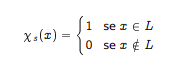
\includegraphics[scale=0.8]{tesi_stile/img/sem1.png}
\end{figure}
Il problema L è \textbf{semidecidibile} se esiste una macchina di Turing M che accetta L, ovvero, per ogni x $\in$ N,
\begin{center}
    M $\downarrow$ x se e solo se x $\in$ L
\end{center}
\textbf{Teorema}\\
Sia L  $\subseteq$ N. Allora le proposizioni seguenti sono equivalenti:
\begin{itemize}
    \item L è semidecidibile
    
    \item L è il dominio di una funzione calcolabile
    
    \item L è vuoto o c’è una funzione totale calcolabile $f : N \mapsto N$ tale che $L = f (N)$
\end{itemize}
\newpage
\subsection{Enumerabilità effettiva}
\textbf{Osservazione}\\
Se $L\neq\emptyset$, la condizione 3 esprime il fatto che esiste una enumerazione effettiva degli elementi di L:
\begin{center}
    f(0),f(1),f(2), . . . , f (n), . . .
\end{center}
\textbf{Dimostrazione}
\begin{enumerate}
    \item L è semidecidibile
    
    \item L è il dominio di una funzione calcolabile
    
    \item L è vuoto o c’è una funzione totale calcolabile $f : N \mapsto N$ tale che $L = f (N)$
\end{enumerate}
L’equivalenza tra 1 e 2 è immediata.\\
Mostriamo che 1 implica 3. Se $L\neq\emptyset$ è accettato dalla macchina di Turing M , allora la seguente procedura infinita produce tutti gli elementi di L (con ripetizioni).\\
\begin{figure}[htp]
    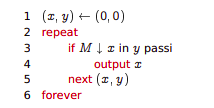
\includegraphics[scale=0.8]{tesi_stile/img/semi2.png}
\end{figure}
(next genera la coppia successiva in una enumerazione di $N x N$)\\
Poniamo $f(x)$ uguale all’($x+1$)-esimo output della procedura precedente.\\
Mostriamo che 3 implica 1. Se $L = f (N)$, allora L è accettato dalla macchina di Turing che esegue il seguente algoritmo.
\begin{figure}[htp]
    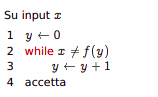
\includegraphics[scale=0.8]{tesi_stile/img/semi3.png}
\end{figure}
\subsection{Insiemi semidecidibili e decidibili}
\textbf{Teorema}\\
Un insieme L è decidibile se e solo se sia L che il suo complemento sono semidecidibili.\\\\
\textbf{Dimostrazione}\\
Se L è decidibile, lo è anche il complemento. Pertanto, sono semidecidibili entrambi.\\
Viceversa, se L e il suo complemento sono accettati dalle macchine di Turing $M$ e $M'$, rispettivamente, la seguente procedura decide L:\\
\begin{figure}[htp]
    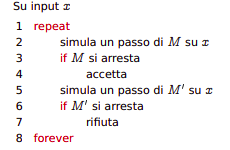
\includegraphics[scale=0.8]{tesi_stile/img/official.png}
\end{figure}\\
\textbf{Esempio}\\
Il problema:
\begin{center}
    K = \{$x \in N | M_x \downarrow x $\}
\end{center}
è semidecidibile ma non decidibile (invero è riducibile al problema dell’arresto, che è semidecidibile in quanto accettato dalla macchina di Turing universale).\\
Pertanto:\\
\begin{center}
    $\overline{k}$ = \{$x \in N | M_x \uparrow x $\}
\end{center}
non è semidecidibile.\\
\textbf{Osservazione}\\
Esistono macchine di Turing M per cui è indecidibile il problema.
\begin{center}
    \{$x \in N | M \downarrow x$\}.
\end{center}
In effetti, qualunque macchina di Turing che accetti un linguaggio semidecidibile ma non decidibile (come, ad es., K ) ha questa proprietà.
\subsection{Il 10 problema di Hilbert}
Data un’equazione Diofantea, determinare se ammette soluzioni intere.\\
Il problema seguente si riduce al decimo problema di Hilbert.\\\\
\textbf{Problema}\\
Data un’equazione Diofantea, determinare se ammette soluzioni in numeri naturali\\\\
\textbf{Dimostrazione}\\
L’equazione
\begin{center}
    $D(x,y,z) = 0$
\end{center}
ha una soluzione naturale se e soltanto se l’equazione.\\
\begin{center}
    $D(x^2_1 + x^2_2 + x^2_3 + x^2_4, y^2_1 + y^2_2 + y^2_3 + y^2_4, z^2_1 + z^2_2 + z^2_3 + z^2_4) = 0$
\end{center}
ha una soluzione intera (per il Teorema dei quattro quadrati di Lagrange).
\subsection{Insiemi diofanteei}
\textbf{Definizione}\\
Un insieme $L \subseteq N$ si dice Diofanteo se esiste un’equazione Diofantea $D(x_0, x_1, . . . , x_m) = 0$ tale che
\begin{center}
    $L = \{a \in N | D(a, x_1, . . . , x_m ) = 0$ ha soluzione\}
\end{center}
\textbf{Osservazione}\\
Una soluzione del 10. problema di Hilbert implicherebbe la decidibilità di tutti gli insiemi Diofantei.\\\\
\textbf{Esempi}\\
L’insieme dei quadrati perfetti è rappresentato da
\begin{center}
    $a - x^2 = 0$
\end{center}
L’insieme dei numeri composti è rappresentato da
\begin{center}
    $a - (x_1 + 2)(x_2 + 2) = 0$
\end{center}
L’insieme dei numeri che non sono potenze di 2 è rappresentato da
\begin{center}
    $a - (2x_1 +3)x_2 = 0$
\end{center}
\textbf{Proposizione}\\
Gli insiemi Diofantei sono semidecidibili. (perchè è semidecidibile il 10. problema di Hilbert)
\subsection{Insiemi Diofantei e insiemi semidecidibili}
\textbf{Osservazione}\\
L’equazione $D(a, x_1, . . . , x_m ) = 0$ ha soluzioni se e solo se ha soluzioni l’equazione:
\begin{center}
    $a = (x_0 + 1)(1 - (D(x_0, x_1, . . . , x_m))2) - 1$
\end{center}
Quindi, un insieme Diofanteo è l’insieme dei valori positivi assunti da un polinomio con variabili in N.\\\\
\textbf{Congettura di M. Davis}\\
\begin{figure}[htp]
    \centering
    
\includegraphics[scale=0.9]{tesi_stile/img/semi6.png}
\end{figure}\\
\textbf{Teorema (M. Davis, H. Putnam, J. Robinson)}\\
Per ogni insieme semidecidibile L esiste un’equazione Diofantea esponenziale E tale che
\begin{center}
    $L = \{a \in N | E ha una soluzione (a, x_1, . . . , x_n )\}$
\end{center}
Un’equazione Diofantea esponenziale è, ad esempio
\begin{center}
    $(x + 1)^{y+2} + x^3 = y^{(x+1)^x}+ y^4$
\end{center}
\subsection{Prova della congettura di Davis}
Come corollario del teorema di Davis, Putnam e Robinson, per provare la congettura di Davis ci si può ridurre al solo insieme:
\begin{center}
    ${(a, b, a^b) | a, b \in N}$
\end{center}
Il fatto che quest’ultimo insieme è Diofanteo è stato definitivamente dimostrato da Y. Matiyasevich (1970).\\\\
\textbf{Teorema (Davis, Putnam, Robinson, Matiyasevich)}\\
Ogni insieme semidecidibile è Diofanteo. Pertanto il 10. problema di Hilbert è indecidibile.\\\\
\textbf{Osservazione}\\
L’intera teoria della computabilità si può riscrivere in termini di equazioni Diofantee.\\\\
\textbf{Problema}\\
Data un’equazione Diofantea, determinare se ammette soluzioni razionali.




